% Compilar con: xelatex decisiones_metodologicas.tex (dos pasadas)
\documentclass[11pt,a4paper]{article}

\usepackage{fontspec}
\setmainfont{Latin Modern Roman}
\usepackage[top=2.4cm,bottom=2.4cm,left=2.6cm,right=2.6cm]{geometry}
\usepackage{amsmath,amssymb}
\usepackage{booktabs,array,longtable}
\usepackage{xcolor}
\usepackage{tikz}
\usepackage{enumitem}
\usepackage{microtype}
\usepackage{fancyhdr}
\usepackage[colorlinks=true,linkcolor=blue!50!black,urlcolor=blue!50!black,pdfborder={0 0 0}]{hyperref}

\renewcommand{\contentsname}{Contenido}
\setlength{\parindent}{0pt}
\setlength{\parskip}{0.55em}
\renewcommand{\arraystretch}{1.15}
\setlist{itemsep=2pt,topsep=2pt}

\pagestyle{fancy}
\fancyhf{}
\fancyhead[L]{\small\textsc{Decisiones metodológicas}}
\fancyhead[R]{\small Clasificación de marcha sagital: control vs.\ PC}
\fancyfoot[C]{\small\thepage}

\newcommand{\termino}[1]{\textbf{#1}}

\title{\textbf{Decisiones metodológicas}\\[0.2em]\large Clasificación de marcha sagital: control vs.\ parálisis cerebral}
\author{Equipo de Investigación EAFIT}
\date{Noviembre de 2026}

\begin{document}
\maketitle
\thispagestyle{fancy}

\begin{center}\small
Documento de apoyo del informe principal (\texttt{informe\_clasificacion\_sagital.pdf}).\\
Explica \emph{qué} se decidió, \emph{qué} se descartó y \emph{por qué}, en términos prácticos.
\end{center}

\section{Contexto en una línea}

Se dispone de 56 niños (17 con parálisis cerebral, 39 controles) y 212 ciclos de marcha. Con tan pocos sujetos, casi todas las decisiones de evaluación giran en torno a una idea: \emph{no engañarnos con resultados que dependen del azar o de datos que el modelo ya vio.}

\section{Resumen de decisiones}

\begin{longtable}{>{\raggedright\arraybackslash}p{2.5cm}>{\raggedright\arraybackslash}p{3.3cm}>{\raggedright\arraybackslash}p{3.2cm}>{\raggedright\arraybackslash}p{4.9cm}}
\toprule
\textbf{Tema} & \textbf{Decisión} & \textbf{Alternativa descartada} & \textbf{Motivo} \\
\midrule
\endhead
Evaluación & Validación cruzada 4 particiones $\times$ 5 repeticiones & Un único reparto 70/15/15 & El test tenía 9 niños y solo 3 casos: un niño cambiaba la sensibilidad 33 puntos. \\
Unidad de reparto & El \textbf{sujeto} & El ciclo & Ciclos del mismo niño son casi iguales; repartirlos filtra información. \\
Peso de cada ciclo & $1/n_s$ y clases balanceadas a nivel sujeto & Pesos por clase a nivel ciclo & Los controles aportan 4.1 ciclos por niño y los casos 3.1. \\
Métrica principal & AUC a nivel paciente & Exactitud por ciclo & Hay 70\,\% de controles: predecir siempre ``control'' ya da 69.6\,\% por sujeto. \\
Umbral de decisión & Fijo en 0.5, sin calibrar, como métrica secundaria & Calibrarlo & Con 17 casos el umbral óptimo es inestable. \\
Incertidumbre & Media $\pm$ DE e IC95\,\% por bootstrap de sujetos & Un único número & Con pocos sujetos hay que mostrar cuánto podría variar. \\
Importancia de variables & Permutación, medida en test & Importancia de Gini & Gini se calcula con datos ya vistos y se reparte mal entre variables correlacionadas. \\
CNN & Detención temprana con validación interna por sujeto & Número fijo de épocas o usar el test & El test no puede intervenir en ningún ajuste. \\
Lectura clínica & No interpretar patrones (equino, \emph{crouch}\dots) & Observaciones clínicas escritas a priori & Pose por video, ángulos aparentemente sin signo y ninguna prueba que las respalde. \\
12 sujetos sin ciclos & Documentar la exclusión & Reconstruir sus ciclos & Decisión del equipo de no abordarlo en esta etapa. \\
\bottomrule
\end{longtable}

\section{Cómo funciona la validación cruzada}

\subsection{Una repetición}

Se barajan los 56 sujetos y se dividen en 4 grupos de unos 14 (cada uno con unos 4 casos y 10 controles: eso es ser \emph{estratificada}). Luego se hacen 4 rondas; en cada una un grupo es \textbf{prueba} y los otros tres son \textbf{entrenamiento}.

\begin{center}
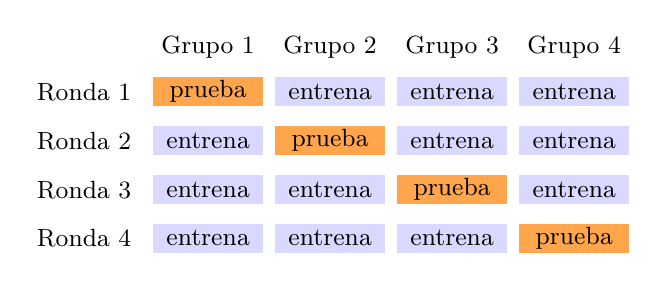
\begin{tikzpicture}[x=1.55cm,y=0.62cm,font=\small]
  \foreach \r in {1,2,3,4} {
    \node[anchor=east] at (0.45,-\r) {Ronda \r};
    \foreach \c in {1,2,3,4} {
      \ifnum\r=\c
        \fill[orange!70] (\c-0.45,-\r-0.3) rectangle (\c+0.45,-\r+0.3);
        \node at (\c,-\r) {prueba};
      \else
        \fill[blue!15] (\c-0.45,-\r-0.3) rectangle (\c+0.45,-\r+0.3);
        \node at (\c,-\r) {entrena};
      \fi
    }
  }
  \foreach \c in {1,2,3,4} { \node at (\c,-0.1) {Grupo \c}; }
\end{tikzpicture}
\end{center}

Al terminar las 4 rondas, \textbf{cada niño fue evaluado exactamente una vez} con un modelo que no lo vio entrenar. El AUC se calcula sobre los 56 niños, no sobre 9.

\subsection{Por qué agrupar por sujeto}

Un niño tiene entre 1 y 6 ciclos, muy parecidos entre sí. Si se repartieran ciclos, el modelo vería algunos de un niño en el entrenamiento y otros del mismo niño en la prueba, y podría ``reconocer al niño'' en lugar de aprender patrones de la enfermedad. Repartiendo sujetos completos eso no ocurre; el código lo verifica con una comprobación explícita.

\subsection{Por qué repetir 5 veces}

El reparto en 4 grupos es aleatorio y otro reparto da otro resultado. Repetirlo con 5 repartos distintos (20 ajustes por modelo) permite ver cuánto depende la métrica de ese azar. De ahí sale el ``$0.79 \pm 0.04$''.

\section{Ponderación por sujeto}

Si un niño tiene 5 ciclos y otro tiene 1, sin ajuste el primero pesaría cinco veces más en el entrenamiento y en las métricas. Cada ciclo recibe un peso proporcional a $1/n_s$ (siendo $n_s$ los ciclos de su sujeto), de modo que \textbf{cada niño aporta lo mismo en total}. Después las dos clases se reescalan para sumar el mismo peso total. Así se corrigen a la vez dos desbalances: ciclos por niño y casos frente a controles.

\section{AUC frente a umbral}

El \termino{AUC} responde: ``si tomo un caso y un control al azar, ¿con qué frecuencia el modelo da mayor probabilidad al caso?''. No depende de ningún corte. Un AUC de 0.5 es el azar. Con 0.79, el modelo acierta el orden en cuatro de cada cinco parejas; \textbf{no} significa 79\,\% de aciertos.

La sensibilidad, la especificidad y la exactitud balanceada sí dependen del \termino{umbral} (aquí 0.5). Ese corte solo es adecuado si las probabilidades están bien calibradas, y las del Random Forest probablemente no lo están: ordena bien, pero casi nunca supera 0.5 para un caso (sensibilidad 0.02). Por eso esas métricas se muestran aparte, rotuladas como ``sin calibrar'', y \textbf{no se usan para comparar modelos}: cada modelo calibra distinto.

\section{Dos tipos de incertidumbre}

\begin{itemize}
\item \textbf{Media $\pm$ DE entre repeticiones:} cuánto cambia el AUC según cómo se repartieron los sujetos.
\item \textbf{IC95\,\% por bootstrap:} cuánto podría cambiar el AUC si hubiera tocado otro grupo de niños (se remuestrean los 56 sujetos con reemplazo miles de veces). Es más ancho porque refleja el tamaño de la muestra.
\end{itemize}

El IC se calcula sobre la probabilidad promediada entre repeticiones, lo que lo hace \textbf{algo optimista}; debe leerse como orientativo. Por eso en la curva ROC se dibujan también las 5 repeticiones por separado.

\section{Importancia por permutación}

Se toma el modelo ya entrenado y un conjunto de prueba con su AUC. Se \textbf{baraja una característica} entre los ciclos (las demás no se tocan) y se recalcula el AUC: si cae mucho, el modelo dependía de esa característica; si no cambia, no la usaba. Se repite 10 veces por característica y en cada una de las 20 particiones.

Se prefirió a la importancia de Gini porque se mide en datos no vistos y no favorece a variables con muchos valores distintos. Su límite: con características muy correlacionadas (media, mínimo, máximo y ROM de una misma señal) puede subestimar a cada una, porque las demás compensan. Aquí la mayor caída fue de 0.03 y casi todas con ruido igual o mayor, así que la lectura es ``ninguna destaca'', no ``las demás no importan''.

\section{Detención temprana de la CNN}

Dentro de cada ronda, la red separa un 20\,\% de los \emph{sujetos} del entrenamiento como mini-validación y deja de entrenar cuando su pérdida no mejora en 10 épocas, conservando el mejor estado. Es un reparto anidado: el conjunto de prueba de la ronda nunca interviene, de modo que el AUC no está inflado por haber ``elegido'' la mejor época mirando el test.

\section{Reproducibilidad}

\begin{itemize}
\item Semilla 42 en el reparto de la validación cruzada; el modelo de cada partición usa la semilla $42+k$.
\item Entorno: Python 3.13, scikit-learn 1.7, PyTorch 2.13 (CPU), NumPy 2.3, pandas 2.3.
\item Dos ejecuciones completas del cuaderno en la misma máquina dieron los mismos AUC (0.790 y 0.649). No se probó en otro entorno; el entrenamiento de la red puede variar levemente entre máquinas.
\item Reejecución, desde la raíz del repositorio:\\
\texttt{\small jupyter nbconvert --to notebook --execute --inplace}\\
\texttt{\small notebooks/sagittal\_control\_vs\_case.ipynb}
\end{itemize}

\section{Qué queda abierto}

\begin{itemize}
\item \textbf{Signo de cadera y rodilla:} no toman valores negativos; verificar si son ángulos sin signo en el procesamiento previo.
\item \textbf{12 sujetos excluidos} (10 casos): recuperarlos es lo que más aumentaría la potencia del estudio.
\item \textbf{Asimetría:} compara ciclos izquierdo y derecho con el mismo índice, que no son el mismo paso; se podría emparejar por cercanía temporal.
\item \textbf{Validación externa:} todos los registros comparten cámara y sesión.
\end{itemize}

\end{document}
